%----------createPackageInModel----------------------------------------
\op
{createPackageInModel}
{Adds a package in a model / under the root element}
{createPackageInModel(Model selectedEObject, String idValue, String nameValue)}
{The model providing the container for the newly created package.}
{
\begin{itemize}
 \item idValue/newID: The identifier of the newly created package 
 \item nameValue/newName: The name of the newly created package
\end{itemize}
}
{There is no package whose name equals the parameter-value of 'newName' (see
\ref{subsec:checkOtherNames})}
{A new package and references to and from
the model will be created. 'selectedModel', as it is shown in the picture,
is a placeholder for the concrete Model which will be delivered via mappings
of the selectedEObject. Also a default value 'public' for the visibility feature
will be set.} \begin{figure}[H]
  \centering
  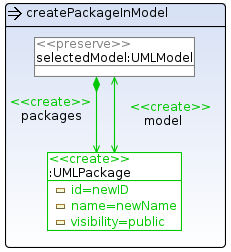
\includegraphics[width=0.4\textwidth]{pics/createPackageInModel.png}    
  \caption{createPackageInModel}
  \label{createPackageInModel}  
\end{figure}

%----------createPackageInPackage----------------------------------------
\op
{createPackageInPackage}
{Adds a package in a package}
{createPackageInPackage(Package selectedEObject, String idValue, String nameValue)}
{The package providing the container for the newly created package.}
{
\begin{itemize}
 \item idValue/newID: The identifier of the newly created package 
 \item nameValue/newName: The name of the newly created package
\end{itemize}
}
{There is no package whose name equals the parameter-value of 'newName' (see
\ref{subsec:checkOtherNames})}
{A new package and references to and from
the super package will be created. 'selectedPackage', as it is shown in the
picture, is a placeholder for the concrete super package which will be delivered
via mappings of the selectedEObject. Also a default value 'public' for the visibility feature
will be set.}
\begin{figure}[H]
  \centering
  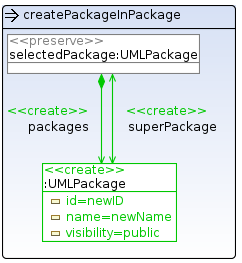
\includegraphics[width=0.4\textwidth]{pics/createPackageInPackage.png}
  \caption{createPackageInPackage}
  \label{createPackageInPackage}
\end{figure}

%----------deletePackage----------------------------------------
\op
{deletePackage}
{Deletes a package}
{deletePackage(Package selectedEObject)}
{The package which should be deleted }
{-}
{-}
{For a better readability this is a simplified version of the
'deletePackage'-transformation and will only cover cases where the
package has no containments and no references to other elements. Such a
complex transformation rule exits but won't be listed here.
\\\\
In this simple version we first of all have to find out from which context type
the selected package should be deleted. For this we have the rule 'containerIsModel', which matches if the
container is a model. If not we can assume that the context is a package since
no other model element can contain a package according to the meta model specification.\\
After we know the context type one of the two variants of the delete-rule
(deletePackageFromModel and deletePackageFromPackage) can be applied.\\\\
Below you can also see the graph of units which explains this process with
an if-then-else structure called 'Conditional Unit'. The selectedEObject is the
placeholder for the context and it will be propagated to the according
parameters in the three rules via the so called 'Parameter Mappings'.

}
\begin{figure}[H]
  \advance\leftskip-1.5cm
  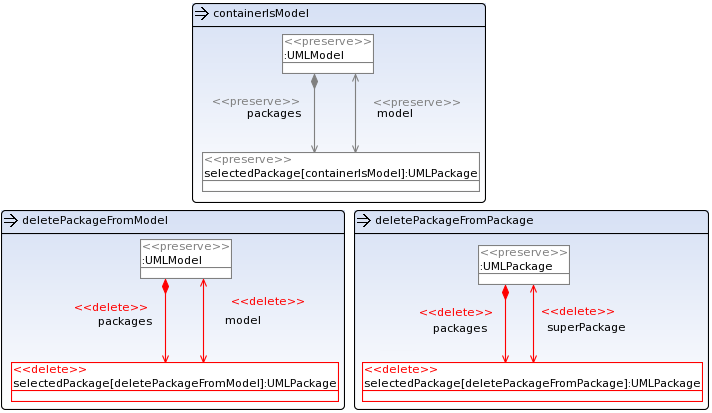
\includegraphics[width=1.2\textwidth]{pics/deletePackage_emptyAndUnreferenced.png}
  \caption{deletePackage}
  \label{deletePackage}
\end{figure}
\begin{figure}[H]
  \centering
  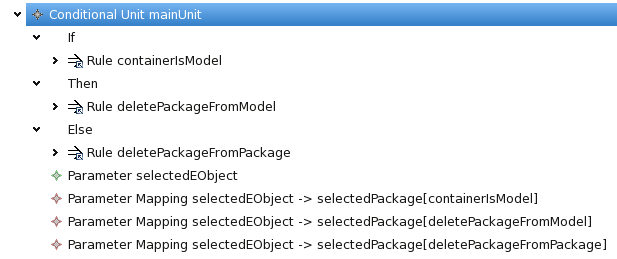
\includegraphics[width=1.0\textwidth]{pics/deletePackage_emptyAndUnreferenced_TreeView.png}
  \caption{deletePackage(UnitView)}
  \label{deletePackage}
\end{figure}
%----------editPackageName----------------------------------------
\op
{editPackageName}
{edits the name of a package}
{editPackageName(Package selectedEObject, String nameValue)}
{The package whose name should be renamed.}
{
\begin{itemize}
 \item nameValue/newName: The new name
\end{itemize}
}
{There is no package whose name equals the parameter-value of 'newName' (see
\ref{subsec:checkOtherNames})}
{The 	\textless\textless create\textgreater\textgreater  -symbol in the image
means that even if the attribute exists its value will be overwritten. 'newName'
is the placeholder for the input name.}
\begin{figure}[H]
  \centering
  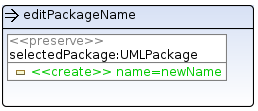
\includegraphics[width=0.4\textwidth]{pics/editPackageName.png}
  \caption{editPackageName}
  \label{editPackageName}
\end{figure}

%----------editPackageVisibility----------------------------------------
\op
{editPackageVisibility}
{edits the visibility of a package}
{editPackageVisibility(Package selectedEObject, Visibility visibilityValue)}
{The package whose visibility should be edited.}
{
\begin{itemize}
 \item visibilityValue/visibility: The new visiblility
\end{itemize}
}
{-}
{The 	\textless\textless create\textgreater\textgreater  -symbol in the image
means that even if the attribute exists its value will be overwritten.
'visibility' is the placeholder for the input visibility.}
\begin{figure}[H]
  \centering
  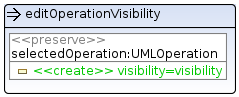
\includegraphics[width=0.4\textwidth]{pics/editPackageVisibility.png}
  \caption{editPackageVisibility}
  \label{addPackage-execute}
\end{figure}

%----------movePackageFromModelToPackage----------------------------------------
\op
{movePackageFromModelToPackage}
{moves a package from a model into package}
{movePackageFromModelToPackage(Package selectedEObject, Package tgt)}
{The package which should be moved.}
{
\begin{itemize}
 \item tgt/targetPackage: the target package
\end{itemize}
}
{There is no package with the same name in the target context (see
\ref{subsec:checkOtherNames})}
{Only the references change}
\begin{figure}[H]
  \centering
  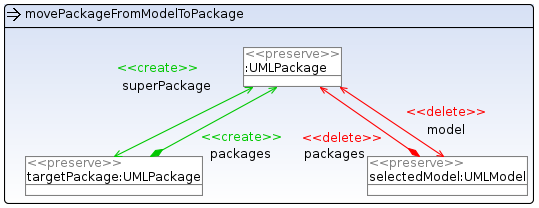
\includegraphics[width=0.8\textwidth]{pics/movePackageFromModelToPackage.png}.
  \caption{movePackageFromModelToPackage}
  \label{movePackageFromModelToPackage}
\end{figure}
%----------movePackageFromModelToPackage----------------------------------------
\op
{movePackageFromPackageToModel}
{moves a package from a package directly under the model}
{movePackageFromPackageToModel(Package selectedEObject, Model tgt)}
{The package which should be moved.}
{
\begin{itemize}
 \item tgt/targetModel: the target model
\end{itemize}
}
{There is no package with the same name in the target context (see
\ref{subsec:checkOtherNames})}
{Only the references change}
\begin{figure}[H]
  \centering
  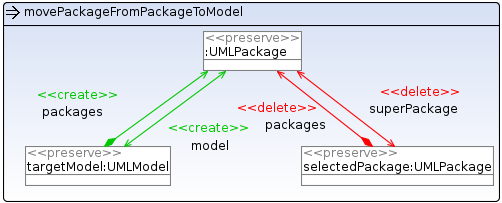
\includegraphics[width=0.7\textwidth]{pics/movePackageFromPackageToModel.png}.
  \caption{movePackageFromPackageToModel}
  \label{movePackageFromPackageToModel}
\end{figure}
%----------movePackageFromModelToPackage----------------------------------------
\op
{movePackageFromPackageToPackage}
{moves a package from a package into another package}
{movePackageFromPackageToPackage(Package selectedEObject, Package tgt)}
{The package which should be moved.}
{
\begin{itemize}
 \item tgt/targetPackage: the target package
\end{itemize}
}
{There is no package with the same name in the target context (see
\ref{subsec:checkOtherNames})}
{Only the references change}
\begin{figure}[H]
  \centering
  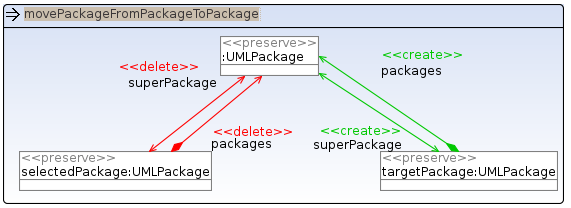
\includegraphics[width=0.9\textwidth]{pics/movePackageFromPackageToPackage.png}.
  \caption{movePackageFromPackageToPackage}
  \label{movePackageFromPackageToPackage}
\end{figure}